%% LaTeX-Beamer template for KIT design
%% by Erik Burger, Christian Hammer
%% title picture by Klaus Krogmann
%%
%% version 2.1
%%
%% mostly compatible to KIT corporate design v2.0
%% http://intranet.kit.edu/gestaltungsrichtlinien.php
%%
%% Problems, bugs and comments to
%% burger@kit.edu

\documentclass[18pt]{beamer}

%% SLIDE FORMAT

% use 'beamerthemekit' for standard 4:3 ratio
% for widescreen slides (16:9), use 'beamerthemekitwide'

\usepackage{templates/beamerthemekit}
% \usepackage{templates/beamerthemekitwide}

\usepackage[utf8]{inputenc}
\usepackage{hyperref}
\usepackage{listings}

%% TITLE PICTURE

% if a custom picture is to be used on the title page, copy it into the 'logos'
% directory, in the line below, replace 'mypicture' with the
% filename (without extension) and uncomment the following line
% (picture proportions: 63 : 20 for standard, 169 : 40 for wide
% *.eps format if you use latex+dvips+ps2pdf,
% *.jpg/*.png/*.pdf if you use pdflatex)

\titleimage{greendrop}

%% TITLE LOGO

% for a custom logo on the front page, copy your file into the 'logos'
% directory, insert the filename in the line below and uncomment it

%\titlelogo{mylogo}

% (*.eps format if you use latex+dvips+ps2pdf,
% *.jpg/*.png/*.pdf if you use pdflatex)

%% TikZ INTEGRATION

% use these packages for PCM symbols and UML classes
% \usepackage{templates/tikzkit}
% \usepackage{templates/tikzuml}

% the presentation starts here

\title[Hello World]{Programmieren: Hello World}
\subtitle{Tutorium 30}
\author{YouniS Bensalah}
\date{October 30, 2015}

\institute{Chair for Software Design and Quality}

% Bibliography

\usepackage[citestyle=authoryear,bibstyle=numeric,hyperref,backend=biber]{biblatex}
\addbibresource{templates/example.bib}
\bibhang1em

\begin{document}

% change the following line to "ngerman" for German style date and logos
\selectlanguage{english}

%title page
\begin{frame}
\titlepage
\end{frame}

%table of contents
\begin{frame}{Heute}
\tableofcontents
\end{frame}

\section{Organisatorisches}

\begin{frame}{Prüfung und Übungsschein}
    \begin{block}{Anmeldung zur Prüfung und zum Übungsschein}
        \begin{itemize}
            \item Campus Management Portal für Studierende
            \begin{itemize}
                \item Informatik, Informationswirtschaft, Mechatronik
                \item \url{https://campus.studium.kit.edu}
            \end{itemize}
            \pause

            \item Blauer Schein
            \begin{itemize}
                \item Alle anderen Studiengänge \dots
                \item Im Studienbüro
                \pause
                \item \textbf{ZEITNAH !}
            \end{itemize}
        \end{itemize}
    \end{block}
\end{frame}

\begin{frame}{Einverständniserklärung}
    \begin{itemize}
        \item Solltet Ihr bereits abgegeben haben.
        \pause
        \item Falls nicht:
        \begin{itemize}
            \item \textbf{ZEITNAH} im \textit{Programmieren-Briefkasten} unterschrieben einwerfen !
            \item Info-Bau (50.34) im 1. UG
        \end{itemize}
    \end{itemize}
\end{frame}

\begin{frame}{Praktomat und ILIAS}
    \begin{block}{Praktomat}
        \begin{itemize}
            \item Kurz einloggen via KIT-Account
            \item \url{https://praktomat.cs.kit.edu/2015\_WS}
            \item Nur aus dem Campus-Netz oder via VPN erreichbar !
        \end{itemize}
    \end{block}
    \pause

    \begin{block}{ILIAS-Forum}
        \begin{itemize}
            \item Kurz einloggen via KIT-Account
            \item \url{https://ilias.studium.kit.edu}
            \item Kurs beitreten
        \end{itemize}
    \end{block}
\end{frame}

\begin{frame}{Folien etc.}
    \begin{itemize}
        \item Vorlesung, Übungsblätter etc.\\ \url{https://sdqweb.ipd.kit.edu/wiki/Vorlesung\_Programmieren\_WS15/16}
        \item Tutorium \\ \url{http://younishd.fr/prog}
    \end{itemize}
\end{frame}

\begin{frame}{Kontakt}
    \begin{itemize}
        \item E-Mail: \url{younis.bensalah@riseup.net}
        \item GPG key: D3D1D9B1\\ \url{http://younishd.fr/stuff/younis.key}
    \end{itemize}
\end{frame}

\section{VPN}

\begin{frame}{VPN}
    \begin{block}{VPN}
        \begin{itemize}
            \item Möglichkeit, von außerhalb (z.B. von zu Hause) eine Verbindung mit dem KIT-Intranet herzustellen
            \item Zugang mit KIT-Account
            \item \url{https://www.scc.kit.edu/dienste/vpn.php}
        \end{itemize}
    \end{block}
\end{frame}

\section{JDK}

\begin{frame}{JDK}
    \begin{block}{JDK Installation}
        \begin{itemize}
            \item Java Development Kit
            \item Version 7 (\textit{nicht} 8)
            \item OpenJDK oder Oracle JDK
            \pause
            \item Linux
            \begin{itemize}
                \item Via package manager
                \item \url{openjdk-7-jdk} oder \url{jdk7-openjdk} oder \dots
            \end{itemize}
            \item Mac OS
            \begin{itemize}
                \item JDK sollte bereits vorinstalliert sein.
            \end{itemize}
            \item Windows
            \begin{itemize}
                \item JDK hier downloaden\\
                \url{http://www.oracle.com/technetwork/java/javase/downloads/jdk7-downloads-1880260.html}
                \item \url{PATH} setzen !
            \end{itemize}
        \end{itemize}
    \end{block}
\end{frame}

\section{Editor}

\begin{frame}{Editor}
    \begin{itemize}
        \pause
        \item Atom
        \pause
        \item Brackets
        \pause
        \item Sublime Text
        \pause
        \item Kate (Linux)
        \pause
        \item TextMate (Mac)
        \pause
        \item Notepad++ (Windows)
        \pause
        \item nano (Linux+Mac)
        \pause
        \item \dots
    \end{itemize}
\end{frame}

\section{Hello World in Java}

\begin{frame}{Hello World in Java}
    \begin{enumerate}
        \item Schreibe folgenden Java-Code in Editor ab
        \item Quelltext-Datei als \texttt{Hello.java} abspeichern
        \item Kompilieren
        \item Ausführen
    \end{enumerate}
\end{frame}

\begin{frame}[fragile]{Hello World in Java}
public class Hello {
    public static void main(String[] args) {
        System.out.println("Hello, world!");
    }
}
\end{frame}

\begin{frame}[fragile]{Hello World in Java}
    \begin{block}{Kompilieren}
        \begin{lstlisting}
% javac Hello.java
        \end{lstlisting}
    \end{block}
    \pause
    \begin{block}{Ausführen}
        \begin{lstlisting}
% java Hello
        \end{lstlisting}
    \end{block}
\end{frame}

\begin{frame}{Under the hood}
    \begin{figure}
        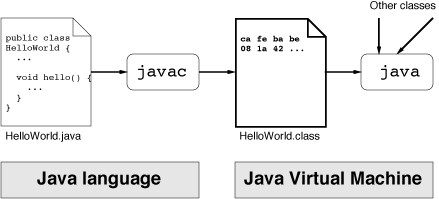
\includegraphics[scale=0.8]{img/jvm.png}
    \end{figure}
\end{frame}

\section{Datentypen, Operationen und Variablen}

\begin{frame}{Primitive Datentypen}
    \begin{itemize}
        \item Ganze Zahlen
        \begin{itemize}
            \item byte {\tiny 8-bit}
            \item short {\tiny 16-bit}
            \item int {\tiny 32-bit}
            \item long {\tiny 64-bit}
        \end{itemize}
        \item Gleitkommazahlen
        \begin{itemize}
            \item float {\tiny 32-bit}
            \item double {\tiny 64-bit}
        \end{itemize}
        \item Wahrheitswerte
        \begin{itemize}
            \item boolean {\tiny 1-bit (\textbf{true} oder \textbf{false})}
        \end{itemize}
        \item Zeichen
        \begin{itemize}
            \item char {\tiny 16-bit (Unicode)}
        \end{itemize}
    \end{itemize}
\end{frame}

\begin{frame}{Datentyp \texttt{String}}
    \begin{itemize}
        \item \texttt{String} repräsentiert Zeichenketten
        \item Konkatenation durch \texttt{+}
        \item \texttt{String} ist eine Klasse !
        \item \texttt{"Hello, world!"}
    \end{itemize}
\end{frame}

\begin{frame}[fragile]{Operationen}
    \begin{itemize}
        \item Arithmetische Operationen
        \begin{verbatim}
+ - * / % ++ --
        \end{verbatim}
        \item Logische Operationen
        \begin{verbatim}
== != < <= >= > && || !
        \end{verbatim}
        \item Bitweise Operationen
        \begin{verbatim}
<< >> >>> & | ^ ~
        \end{verbatim}
    \end{itemize}
\end{frame}

\begin{frame}{Variablen}
    \begin{itemize}
        \item \textbf{Variable} ist Bezeichner für eine Stelle im Speicher
        \pause
        \item \texttt{total = quantity * price;}\\ ist angenehmer als \\ \texttt{0x9DF1346C = 0x89EA24BF * 0x289D0A1B;}
        \pause
        \item \textbf{Deklaration}\\ \texttt{int answer;}
        \item \textbf{Zuweisung} mit \texttt{=} Operator\\ \texttt{answer = 42;}
        \pause
        \item Oder kurz:\\ \texttt{int answer = 42;}
        \pause
        \item \textbf{Tipp:} Immer sofort bei der Deklaration auch einen Wert zuweisen.
    \end{itemize}
\end{frame}

\section{Kontrollflussanweisungen}

\begin{frame}[fragile]{Kontrollflussanweisungen}
    \begin{block}{\texttt{if}}
        \begin{itemize}
            \item Wenn \textit{Kondition} dann \textit{Anweisungen} \dots
        \end{itemize}
    \end{block}
    \pause
    \begin{exampleblock}{Beispiel}
            \begin{lstlisting}[language=Java]
if (semester == 1) {
    System.out.println("Hallo Ersti !");
}
            \end{lstlisting}
    \end{exampleblock}
\end{frame}

\begin{frame}[fragile]{Kontrollflussanweisungen}
    \begin{block}{\texttt{if}}
        \begin{itemize}
            \item Wenn \textit{Kondition} dann \textit{Anweisungen} \dots sonst \textit{Anweisungen} \dots
        \end{itemize}
    \end{block}
    \pause
    \begin{exampleblock}{Beispiel}
            \begin{lstlisting}[language=Java]
if (semester == 1) {
    System.out.println("Hallo Ersti !");
} else {
    System.out.println("Hallo Student !");
}
            \end{lstlisting}
    \end{exampleblock}
\end{frame}

\begin{frame}[fragile]{Kontrollflussanweisungen}
    \begin{block}{\texttt{switch}}
        \begin{itemize}
            \item Fallunterscheidung
            \item Alle \texttt{case} müssen konstant sein !
            \item Nur für Typ \texttt{char, byte, short, int} oder \texttt{String} oder \texttt{enum} definiert !
        \end{itemize}
    \end{block}
\end{frame}

\begin{frame}[fragile]{Kontrollflussanweisungen}
    \begin{exampleblock}{Beispiel}
        \begin{lstlisting}[language=Java,basicstyle=\tiny]
switch (semester) {
case 1:
    System.out.println("Hallo Ersti !");
    break;
case 2:
    System.out.println("Hallo Zweiti !");
    break;
case 3:
    System.out.println("Hallo Dritti !");
    break;
case 4:
    System.out.println("Hallo Vierti !");
    break;
case 5:
    System.out.println("Hallo Fuenfti !");
    break;
case 6:
    System.out.println("Hallo Sechsti !");
    break;
default:
    System.out.println("Hallo Student !");
}
        \end{lstlisting}
    \end{exampleblock}
\end{frame}

\begin{frame}[fragile]{Kontrollflussanweisungen}
    \begin{block}{\texttt{while}}
        \begin{itemize}
            \item Solange \textit{Kondition} : \textit{Anweisungen} \dots
        \end{itemize}
    \end{block}
    \pause
    \begin{exampleblock}{Beispiel}
            \begin{lstlisting}[language=Java]
while (semester < 9000) {
    System.out.println(
        "Dieses Semester lerne ich wirklich...");
    semester++;
}
            \end{lstlisting}
    \end{exampleblock}
\end{frame}

\begin{frame}[fragile]{Kontrollflussanweisungen}
    \begin{block}{\texttt{for}}
        \begin{itemize}
            \item Für \texttt{i} von \textit{Start} bis \textit{Ende} : \textit{Anweisungen} \dots
        \end{itemize}
    \end{block}
    \pause
    \begin{exampleblock}{Beispiel}
            \begin{lstlisting}[language=Java]
for (int i=1; i < 9000; i++) {
    System.out.println(
        "Oh, ich bin schon im " + i + ". Semester !");
}
            \end{lstlisting}
    \end{exampleblock}
\end{frame}

\appendix
\beginbackup

\begin{frame}{Read the fine manual \dots}
    \begin{itemize}
        \item \textbf{Primitive Data Types} \url{https://docs.oracle.com/javase/tutorial/java/nutsandbolts/datatypes.html}
        \item \textbf{Operators} \url{https://docs.oracle.com/javase/tutorial/java/nutsandbolts/operators.html}
        \item \textbf{Variables} \url{https://docs.oracle.com/javase/tutorial/java/nutsandbolts/variables.html}
        \item \textbf{Control Flow Statements} \url{https://docs.oracle.com/javase/tutorial/java/nutsandbolts/flow.html}
    \end{itemize}
\end{frame}

\begin{frame}{Nicht vergessen !!!!!!!!!!!!!!!!!!11111!!!}
    \begin{alertblock}{Nicht vergessen !!!!!!!!!!!!!!!!!!11111!!!}
        \begin{itemize}
        \item Anmeldung zur Prüfung und zum Übungsschein
        \item Einverständniserklärung
        \item Praktomat
        \item ILIAS
        \end{itemize}
    \end{alertblock}
\end{frame}

\begin{frame}{Bis nächste Woche !}
    \begin{figure}
        
\includegraphics[scale=0.5]{img/compiling.png}
    \end{figure}
    \href{https://xkcd.com/303/}{[xkcd]}
\end{frame}

\backupend

\end{document}
